\documentclass{tufte-handout}

\title{Föreläsning 7: Dyck-stigar och Catalantal $\cdot$ 1MA020}

\author[Vilhelm Agdur]{Vilhelm Agdur\thanks{\href{mailto:vilhelm.agdur@math.uu.se}{\nolinkurl{vilhelm.agdur@math.uu.se}}}}

\date{14 februari 2023}


%\geometry{showframe} % display margins for debugging page layout

\usepackage{graphicx} % allow embedded images
  \setkeys{Gin}{width=\linewidth,totalheight=\textheight,keepaspectratio}
  \graphicspath{{graphics/}} % set of paths to search for images
\usepackage{amsmath}  % extended mathematics
\usepackage{booktabs} % book-quality tables
\usepackage{units}    % non-stacked fractions and better unit spacing
\usepackage{multicol} % multiple column layout facilities
\usepackage{lipsum}   % filler text
\usepackage{fancyvrb} % extended verbatim environments
  \fvset{fontsize=\normalsize}% default font size for fancy-verbatim environments
\usepackage{import}
\usepackage{pdfpages}
\usepackage{transparent}
\usepackage{xcolor}
\usepackage{enumitem}
\usepackage{amssymb}
\usepackage{mathtools}
\usepackage[framemethod=TikZ]{mdframed}
\usepackage{hyperref}
%\usepackage{pgfplots}
\usepackage{tikz}
\usepackage{bbm}
\usepackage{mathrsfs}
\usetikzlibrary{automata, positioning, arrows}
\usetikzlibrary{arrows.meta}

\usepackage{color,soul} % Highlights for text

% Standardize command font styles and environments
\newcommand{\doccmd}[1]{\texttt{\textbackslash#1}}% command name -- adds backslash automatically
\newcommand{\docopt}[1]{\ensuremath{\langle}\textrm{\textit{#1}}\ensuremath{\rangle}}% optional command argument
\newcommand{\docarg}[1]{\textrm{\textit{#1}}}% (required) command argument
\newcommand{\docenv}[1]{\textsf{#1}}% environment name
\newcommand{\docpkg}[1]{\texttt{#1}}% package name
\newcommand{\doccls}[1]{\texttt{#1}}% document class name
\newcommand{\docclsopt}[1]{\texttt{#1}}% document class option name
\def\gring{\mathbb{G}}
\def\H{\mathbb{H}}
\def\ora{\overrightarrow}
\def\Lrarr{\Leftrightarrow}
\def\Ln#1{\text{Ln}\left(#1\right)}
\newenvironment{docspec}{\begin{quote}\noindent}{\end{quote}}% command specification environment

\include{mathcommands.extratex}

\begin{document}

\definecolor{darkgreen}{rgb}{0.0627, 0.4588, 0.1451}

\maketitle% this prints the handout title, author, and date

\begin{abstract}
\noindent
Vi introducerar Dyck-stigar, och härleder en rekursion för deras antal. Sedan använder vi rekursionen för att hitta en genererande funktion, och använder genererande funktionen för att ge en explicit formel för deras antal.

Efter det ger vi ett kombinatoriskt bevis för vår formel för antalet Dyck-stigar, som är betydligt kortare.

Slutligen ger vi två till exempel på saker som räknas av Catalantalen.
\end{abstract}

\section{Dyck-stigarr}

\begin{definition}
    En \emph{gitterstig} på $\Z^2$ av längd $n$ mellan $a$ och $b$ börjar i punkten $a$ och tar sig sedan till punkten $b$ med $n$ stycken steg, som kan vara upp, ner, höger, eller vänster.\sidenote[][-0.3cm]{Vi kan betrakta en sådan stig som ett ord av längd $n$ ur alfabetet $\{U,N,H,V\}$, tillsammans med en startpunkt.}

    \begin{figure}
        \centering
        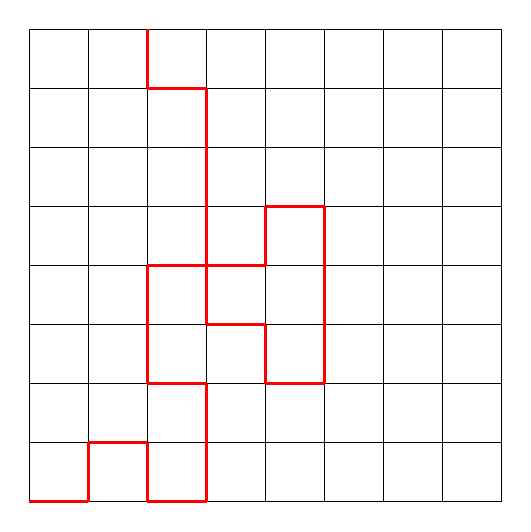
\begin{tikzpicture}
          \draw[step=.75cm] (0,0) grid (6cm,6cm);
          \draw[red, very thick] (0,0) -- (.75cm,0);
          \draw[red, very thick] (.75cm,0) -- (.75cm,.75cm);
          \draw[red, very thick] (.75cm,.75cm) -- (2*.75cm,.75cm);
          \draw[red, very thick] (2*.75cm,.75cm) -- (2*.75cm,0);
          \draw[red, very thick] (2*.75cm,0) -- (3*.75cm,0);
          \draw[red, very thick] (3*.75cm,0) -- (3*.75cm,.75cm);
          \draw[red, very thick] (3*.75cm,.75cm) -- (3*.75cm,2*.75cm);
          \draw[red, very thick] (3*.75cm,2*.75cm) -- (2*.75cm,2*.75cm);
          \draw[red, very thick] (2*.75cm,2*.75cm) -- (2*.75cm,4*.75cm);
          \draw[red, very thick] (2*.75cm,4*.75cm) -- (4*.75cm,4*.75cm);
          \draw[red, very thick] (4*.75cm,4*.75cm) -- (4*.75cm,5*.75cm);
          \draw[red, very thick] (4*.75cm,5*.75cm) -- (5*.75cm,5*.75cm);
          \draw[red, very thick] (5*.75cm,5*.75cm) -- (5*.75cm,2*.75cm);
          \draw[red, very thick] (5*.75cm,2*.75cm) -- (4*.75cm,2*.75cm);
          \draw[red, very thick] (4*.75cm,2*.75cm) -- (4*.75cm,3*.75cm);
          \draw[red, very thick] (4*.75cm,3*.75cm) -- (3*.75cm,3*.75cm);
          \draw[red, very thick] (3*.75cm,3*.75cm) -- (3*.75cm,7*.75cm);
          \draw[red, very thick] (3*.75cm,7*.75cm) -- (2*.75cm,7*.75cm);
          \draw[red, very thick] (2*.75cm,7*.75cm) -- (2*.75cm,8*.75cm);
        \end{tikzpicture}
        \caption{En gitterstig av längd $28$ från $(0,0)$ till $(2,8)$.}
    \end{figure} 
\end{definition}


Det finns uppenbarligen $4^n$ gitterstigar av längd $n$ med en given startpunkt, om vi inte kräver att den skall sluta i någon given punkt.

\begin{definition}
    En \emph{uppåt-höger-stig} på $\Z^2$ från $a$ till $b$ är en gitterstig mellan $a$ och $b$ som enbart tar steg uppåt och åt höger.\sidenote[][]{I tolkningen av stigar som ord är alltså dessa ord ur det mindre alfabetet $\{U,H\}$.}
\end{definition}
\begin{figure}[hbt!]
    \centering
    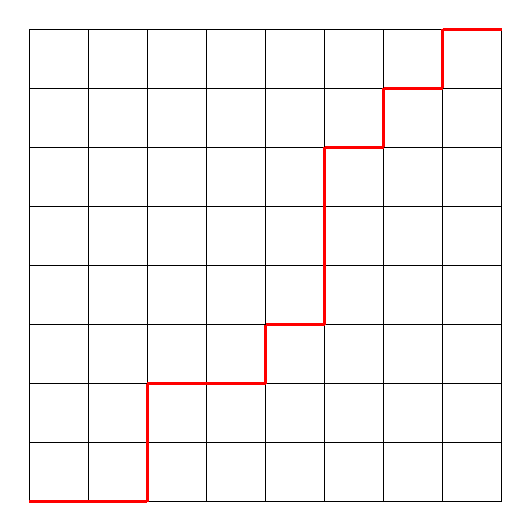
\begin{tikzpicture}
      \draw[step=.75cm] (0,0) grid (6cm,6cm);
      \draw[red, very thick] (0,0) -- (2*.75cm,0);
      \draw[red, very thick] (2*.75cm,0) -- (2*.75cm,2*.75cm);
      \draw[red, very thick] (2*.75cm,2*.75cm) -- (4*.75cm,2*.75cm);
      \draw[red, very thick] (4*.75cm,2*.75cm) -- (4*.75cm,3*.75cm);
      \draw[red, very thick] (4*.75cm,3*.75cm) -- (5*.75cm,3*.75cm);
      \draw[red, very thick] (5*.75cm,3*.75cm) -- (5*.75cm,6*.75cm);
      \draw[red, very thick] (5*.75cm,6*.75cm) -- (6*.75cm,6*.75cm);
      \draw[red, very thick] (6*.75cm,6*.75cm) -- (6*.75cm,7*.75cm);
      \draw[red, very thick] (6*.75cm,7*.75cm) -- (7*.75cm,7*.75cm);
      \draw[red, very thick] (7*.75cm,7*.75cm) -- (7*.75cm,8*.75cm);
      \draw[red, very thick] (7*.75cm,8*.75cm) -- (8*.75cm,8*.75cm);
    \end{tikzpicture}
    \caption{En uppåt-höger-stig från $(0,0)$ till $(8,8)$ av längd sexton.}
\end{figure}

Notera att till skillnad från allmänna gitterstigar bestäms en uppåt-höger-stigs längd av dess start och slutpunkt, eftersom den inte kan ta några omvägar eller gå baklänges. En stig från $(0,0)$ till $(a,b)$ kommer alltid att ta precis $a$ steg uppåt och $b$ steg till höger, det enda som kan variera är i vilken ording stegen tas.

Alltså ges det totala antalet uppåt-höger-stigar från $(0,0)$ till $(a,b)$ av $\binom{a+b}{a}$, eftersom det är antalet sätt att välja de $a$ ställen vi tar ett steg höger av totalt $a+b$ steg.

\begin{definition}
    En Dyck-stig av längd $2n$ är en uppåt-höger-stig från $(0,0)$ till $(n,n)$ som aldrig går under diagonalen.\par
\end{definition}
\begin{figure}[hbt!]
    \centering
    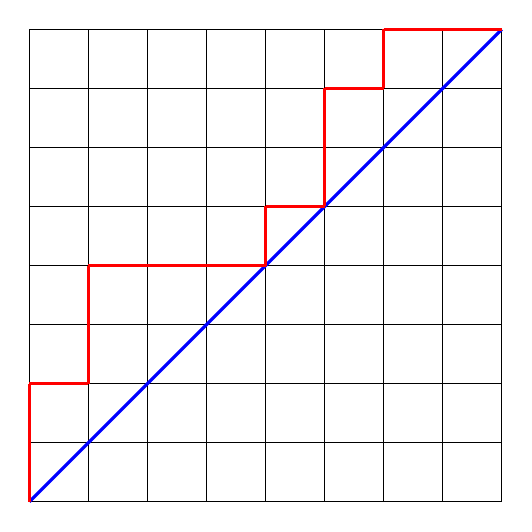
\begin{tikzpicture}
      \draw[step=.75cm] (0,0) grid (6cm,6cm);
      \draw[blue, very thick] (0,0) -- (6cm,6cm);
      \draw[red, very thick] (0,0) -- (0,2*.75cm);
      \draw[red, very thick] (0,2*.75cm) -- (1*.75cm,2*.75cm);
      \draw[red, very thick] (1*.75cm,2*.75cm) -- (1*.75cm,4*.75cm);
      \draw[red, very thick] (1*.75cm,4*.75cm) -- (4*.75cm,4*.75cm);
      \draw[red, very thick] (4*.75cm,4*.75cm) -- (4*.75cm,5*.75cm);
      \draw[red, very thick] (4*.75cm,5*.75cm) -- (5*.75cm,5*.75cm);
      \draw[red, very thick] (5*.75cm,5*.75cm) -- (5*.75cm,7*.75cm);
      \draw[red, very thick] (5*.75cm,7*.75cm) -- (6*.75cm,7*.75cm);
      \draw[red, very thick] (6*.75cm,7*.75cm) -- (6*.75cm,8*.75cm);
      \draw[red, very thick] (6*.75cm,8*.75cm) -- (8*.75cm,8*.75cm);
    \end{tikzpicture}
    \caption{En Dyck-stig av längd sexton.}
\end{figure}

Notera att en Dyck-stig alltid måste börja med ett steg uppåt och sluta med ett steg åt höger, eftersom den annars ju hade varit under diagonalen.\par
\vspace{.2cm}
 Om vi roterar figuren 45 grader medurs noterar vi att vi får något som ser ut som bergskedjor. Detta är ett vanligt sätt att se Dyck-stigar.\par
\vspace{.2cm}
 \begin{figure}[hbt!]
    \centering
    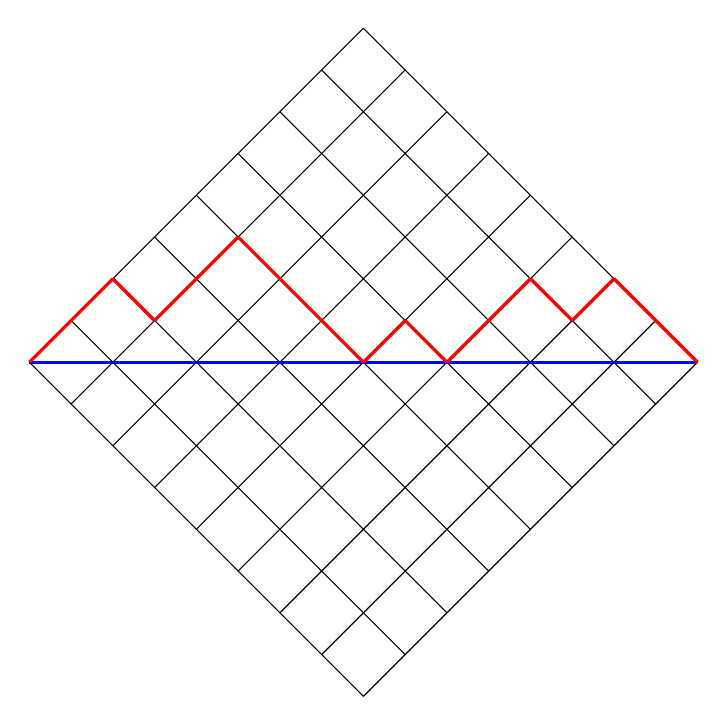
\begin{tikzpicture}[rotate=-45]
      \draw[step=.75cm] (0,0) grid (6cm,6cm);
      \draw[blue, very thick] (0,0) -- (6cm,6cm);
      \draw[red, very thick] (0,0) -- (0,2*.75cm);
      \draw[red, very thick] (0,2*.75cm) -- (1*.75cm,2*.75cm);
      \draw[red, very thick] (1*.75cm,2*.75cm) -- (1*.75cm,4*.75cm);
      \draw[red, very thick] (1*.75cm,4*.75cm) -- (4*.75cm,4*.75cm);
      \draw[red, very thick] (4*.75cm,4*.75cm) -- (4*.75cm,5*.75cm);
      \draw[red, very thick] (4*.75cm,5*.75cm) -- (5*.75cm,5*.75cm);
      \draw[red, very thick] (5*.75cm,5*.75cm) -- (5*.75cm,7*.75cm);
      \draw[red, very thick] (5*.75cm,7*.75cm) -- (6*.75cm,7*.75cm);
      \draw[red, very thick] (6*.75cm,7*.75cm) -- (6*.75cm,8*.75cm);
      \draw[red, very thick] (6*.75cm,8*.75cm) -- (8*.75cm,8*.75cm);
    \end{tikzpicture}
    \caption{Roterad Dyck-stig ser ut som bergskedjor.\par\noindent Denna skulle ha sträng $uuduuddduduududd$.}
  \end{figure}\par
  \vspace{.2cm}
 Ett användbart trick att använda sig av är att uppåt-höger-stigar (eller uppåt-neråt, om man tittar på bergskedjorna) kan översättas till strängar.\par
 \noindent Om vi låter $u$ signalera ``uppåt'' och $h$ signalera ``höger'', blir exempelvis Figur 3 följande:
 \begin{equation*}
   \begin{gathered}
     uuhuuhhhuhuuhuhh
   \end{gathered}
 \end{equation*}
  \par
  \vspace{.2cm}
Hur många Dyck-stigar finns det av varje given längd? Vi kan använda vår observation om att de alltid börjar med ett upp-steg för att ge en rekursion för detta antal:

\begin{lemma}\label{dyck_path_recursion_lemma}
    Låt $d_n$ beteckna antalet Dyck-stigar av längd $2n$. Då gäller det för alla $n \geq 0$ att
    $$d_{n+1} = \sum_{k=0}^{n} d_k d_{n-k}$$
    och $d_0 = 1$.\sidenote[][]{Antalet ord av längd noll anser vi vara ett, eftersom det bara finns ett sätt att välja ett sådant.}

    \begin{proof}
     Om vi låtsas vara stigen i punkten $(0,0)$ som ska gå till $(n,n)$ kanske vi kan klura ut vilka verktyg vi ska använda som vi lärt oss i kursen.\par
     \noindent I varje steg har vi 2 val, upp eller höger. Samtidigt beror vårat val på föregående val, eftersom vi måste hålla oss över diagonalen. Det låter rekursivt! Hittar vi ett rekursivt förhållande så har vi de kraftfulla verktygen \emph{genererande funktioner} som kan ge oss något mer konkret.\clearpage
     \begin{figure}[hbt!]
          \centering
          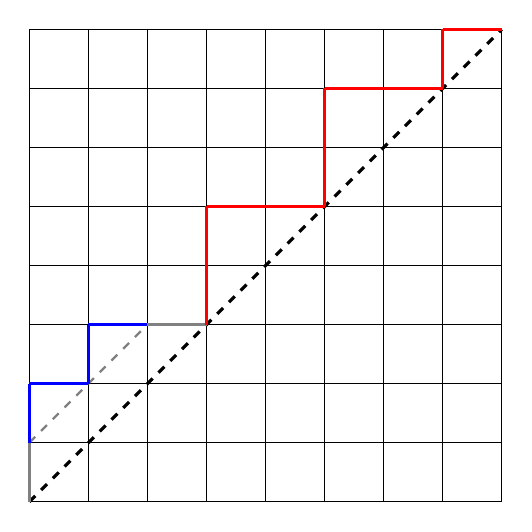
\begin{tikzpicture}
            \draw[step=.75cm] (0,0) grid (6cm,6cm);
            \draw[black,very thick,dashed] (0,0) -- (6cm,6cm);
            \draw[gray,very thick] (0,0) -- (0,.75cm);
            \draw[gray,thick,dashed] (0,.75cm) -- (2*.75cm, 3*.75cm);
            \draw[gray,very thick] (2*.75cm, 3*.75cm) -- (3*.75cm, 3*.75cm);
            \draw[blue, very thick] (0,.75cm) -- (0,2*.75cm);
            \draw[blue, very thick] (0,2*.75cm) -- (.75cm,2*.75cm);
            \draw[blue, very thick] (.75cm,2*.75cm) -- (.75cm,3*.75cm);
            \draw[blue, very thick] (.75cm,3*.75cm) -- (2*.75cm,3*.75cm);
            \draw[red, very thick] (3*.75cm,3*.75cm) -- (3*.75cm,5*.75cm);
            \draw[red, very thick] (3*.75cm,5*.75cm) -- (5*.75cm,5*.75cm);
            \draw[red, very thick] (5*.75cm,5*.75cm) -- (5*.75cm,7*.75cm);
            \draw[red, very thick] (5*.75cm,7*.75cm) -- (7*.75cm,7*.75cm);
            \draw[red, very thick] (7*.75cm,7*.75cm) -- (7*.75cm,8*.75cm);
            \draw[red, very thick] (7*.75cm,8*.75cm) -- (8*.75cm,8*.75cm);
          \end{tikzpicture}
          \caption{En illustration av vår uppdelning av en Dyck-stig i gråa, blåa, och röda steg.}
      \end{figure}
        Överväg en Dyck-stig av längd $2(n+1)$. Vi kan dela upp den i två kortare Dyck-stigar som följer: Den börjar med ett upp-steg, som vi färgar grått. Sedan fortsätter den i ett tag tills den träffar diagonalen för första gången. Vi färgar alla steg innan det steg i vilken den träffar diagonalen blåa, och steget i vilken den träffar diagonalen grått. Sedan färgar vi resten av stegen röda.

        Vi hävdar att de blå stegen utgör en Dyck-stig av längd $2k$ för något $0 \leq k \leq n$, och de röda stegen utgör en Dyck-stig av längd $2(n-k)$, så att vi tillsammans med de två gråa stegen har totalt $2k + 2(n-k) + 2 = 2(n+1)$ steg. Ekvivalent, i tolkningen av stigar som ord, så säger vi att ordet för stigen vi började med kan skrivas som
        $$\underbrace{U}_{\text{Start}}\overbrace{w_1}^{\text{Blå}}\underbrace{H}_{\text{Grå}}\overbrace{w_2}^{\text{Röd}}$$
        för två kortare\sidenote[][]{Det är tillåtet att de är av längd noll.} Dyck-stigar $w_1$ och $w_2$.

        Vi kan välja $k$ fritt mellan $0$ och $n$, och vi kan sedan välja våra två kortare Dyck-stigar helt fritt så länge de har rätt längd, så multiplikations- och additionsprincipen ger oss att vi kan totalt välja på
        $$\sum_{k=0}^{n} d_k d_{n-k}$$
        sätt, vilket är vad vi ville bevisa.
    \end{proof}
\end{lemma}

Den uppmärksamme bland er kanske redan känt igen att den här rekursionen säger något om en faltning -- specifikt säger den att
$$d_{n+1} = (d * d)_n,$$
vilket ser ut som något vi borde kunna använda för att räkna ut genererande funktionen av den här följden.

\begin{proposition}
    Den genererande funktionen för $\{d_k\}_{k=0}^\infty$, antalet Dyck-stigar, är
    $$F_d(x) = \frac{1 - \sqrt{1 - 4x}}{2x}.$$

    \begin{proof}
        Vi observerar att Lemma \ref{dyck_path_recursion_lemma} ger oss att för alla $n \geq 0$
        $$d_{n+1} = (d*d)_n,$$
        så om vi tar genererande funktioner av bägge sidorna ser vi att vänster led blir
        $$\sum_{n=0}^{\infty}d_{n+1}x^n = \frac{1}{x}\sum_{n=0}^{\infty} d_n x^{n+1} = \frac{F_d(x) - 1}{x}$$ %även fast n=0 ger 0, kan det vara pedagogiskt att behålla 0:te indexet
        och höger led blir
        $$F_{d * d}(x) = F_d(x)^2$$
        så att vi har att
        \begin{equation*}
          \begin{gathered}
            F_d(x)^2 = \dfrac{F_d(x)-1}{x}\\
            \Lrarr xF_d(x)^2 = F_d(x)-1\\
            \Lrarr F_d(x) = x F_d(x)^2 + 1.
          \end{gathered}
        \end{equation*}

        Det här är ju bara en vanlig andragradsekvation som vi kan lösa för $F_d$, och få att
        $$F_d(x) = \frac{1 \pm \sqrt{1 - 4x}}{2x}.$$

        Det enda som återstår är att se om den rätta lösningen har ett plus- eller minustecken. Sättet vi ser detta på är att vi vet vad den skall ta för värde i en specifik punkt -- vi vet nämligen att antalet stigar mellan $(0,0)$ och $(0,0)$ är 1
        $$F_d(0) = \sum_{k=0}^{\infty} d_k 0^k = d_0 = 1$$
        så funktionen måste vara ett i noll.

        Vi undersöker vad som händer i $+$ resp. $-$ fallen:
        $$\lim_{x \to 0} \frac{1 - \sqrt{1 - 4x}}{2x} = 1$$
        medan gränsvärdet
        $$\lim_{x \to 0} \frac{1 + \sqrt{1 - 4x}}{2x}$$
        inte existerar. Alltså måste den korrekta lösningen vara med minustecknet, såsom önskat.
    \end{proof}
\end{proposition}

Så, hittills har vi definierat våra Dyck-stigar, listat ut en rekursion för deras antal, och använt denna rekursion för att härleda en genererande funktion. Kan vi använda denna genererande funktion för att härleda en explicit formel för antalet Dyck-stigar?

Svaret på den frågan är ja, men det kräver ett lemma vi inte sett ännu.

\section{Newtons binomialsats, och en explicit formel för $d_n$}

\begin{definition}
    För varje $x\in \R$ och varje $k \in \Z^{\geq 0}$ ges den \emph{fallande fakulteten} $x^{\underline{k}}$ av\sidenote[][]{Så produkten har $k$ termer. I fallet med $k=0$ får vi en tom produkt, vilket vi konventionellt anser är ett, så $x^{\underline{0}} = x^{\overline{0}} = 1$ för alla $x$.}
    $$x^{\underline{k}} = x(x-1)(x-2)\ldots(x-k+1)$$
    och den \emph{stigande fakulteten} $x^{\overline{k}}$ av
    $$x^{\overline{k}} = x(x+1)(x+2)\ldots(x+k-1).$$

    Om $x$ är ett heltal ges alltså $x^{\underline{k}}$ av $\frac{x!}{(x-k)!}$ och $x^{\overline{k}}$ av $\frac{(x+k-1)!}{(x-1)!}$.\par
    \vspace{.2cm}
    Notera att $x^{\underline{k}} = (x-k+1)^{\overline{k}}$
\end{definition}

Vi kan särskilt notera att när $x$ är ett heltal ges antalet permutationer av längd $k$ ur ett alfabete med $x$ bokstäver alltså av $x^{\underline{k}}$, och således har vi också att
$$\binom{x}{k} = \frac{x^{\underline{k}}}{k!}$$
för alla heltal $x$ och $k$. Men detta uttrycket är ju helt väldefinierat även om $x$ inte är ett heltal, vilket motiverar oss att göra följande definition:

\begin{definition}
    För alla $x \in \R$ och $k \in \Z^{\geq 0}$ säger vi att
    $$\binom{x}{k} = \frac{x^{\underline{k}}}{k!}.$$
\end{definition}

Anledningen att vi gör allt detta arbetet är att det låter oss generalisera binomialsatsen även till potenser som inte är heltal, såsom Newton upptäckte.

\begin{theorem}[Newtons binomialsats]
    För alla $x$ och $y$ och $r \in \R$ gäller det att
    $$(x + y)^r = \sum_{k=0}^{\infty} \binom{x}{k} x^{r-k} y^k$$

    \begin{proof}
        Taylorutveckla.\sidenote[][]{Ett bevis återfinns lätt med google, men eftersom det inte egentligen har något med kombinatorik att göra utelämnar vi det i denna kursen.}
    \end{proof}
\end{theorem}

Låt oss nu tillämpa vår nya kunskap på Dyckstigarna. Eftersom den genererande funktionen vi fann för deras antal involverade en kvadratrot kommer vi ju vilja tillämpa Newtons binomialsats i fallet med $r = \frac{1}{2}$, så låt oss börja med ett lemma om vad som händer i just det fallet.

\begin{proposition}\label{ugly_dyck_path_formula}
    Antalet Dyck-stigar av längd $2n$, $d_n$, ges av
    $$d_n = 2 (-1)^{n+1}\binom{1/2}{n+1} 4^n.$$

    \begin{proof}
        Vi vet att den genererande funktionen för denna följd ges av
        $$F_d(x) = \sum_{k=0}^{\infty} d_k x^k = \frac{1 - \sqrt{1 - 4x}}{2x}$$
        så vi behöver serieutveckla detta uttryck.

        Newtons binomialsats säger oss att
        $$\sqrt{1 + y} = \sum_{k=0}^{\infty} \binom{1/2}{k} y^k$$
        så om vi sätter in $y = -4x$ får vi att
        $$\sqrt{1 - 4x} = \sum_{k=0}^{\infty} (-1)^k \binom{1/2}{k} 4^k x^k.$$
        
        När $k=0$ så blir $\binom{1/2}{0} = \frac{(1/2)^{\underline{0}}}{0!} = \frac{1}{1}$, och alltså är hela nollte termen lika med ett. Så alltså gäller det att
        \begin{align*}
            \frac{1 - \sqrt{1 - 4x}}{2x} &= \frac{\sum_{k=1}^{\infty} (-1)^k \binom{1/2}{k} 4^k x^k}{2x}\\
            &= \sum_{k=1}^{\infty} 2(-1)^k \binom{1/2}{k} 4^{k-1} x^{k-1}\\
            &= \sum_{k=0}^{\infty} 2 (-1)^{k+1}\binom{1/2}{k+1} 4^k x^k
        \end{align*}
        vilket genom att jämföra koefficienter ger oss resultatet.
    \end{proof}
\end{proposition}

Så vi har hittat \emph{en} formel, men den är inte särskilt vacker. Även om vi intellektuellt vet att den borde ge oss heltal är det inte alls uppenbart, med den fraktionella binomialkoefficienten och allt.

Kan vi hitta en vackrare formel? Svaret är ja, och det finns flera sätt för oss att göra det. Om vi hade haft mer uthållighet med krångliga räkningar hade vi kunna bevisa följande lemma, vilket låter oss förenkla uttrycket vi fick i Proposition \ref{ugly_dyck_path_formula}:

\begin{lemma}\label{lemma_onehalf_binom_coeff}
    Det gäller att
    $$\binom{1/2}{n} = \frac{(-1)^{n+1}}{4^n(2n-1)}\binom{2n}{n}.$$
    \begin{proof}
        Utelämnas. Om du verkligen vill se en räkning för detta finns det ett bevis för något snarlikt, som borde gå att förenkla till detta, på stackexchange.\cite{dyck_path_stackexchange}
    \end{proof}
\end{lemma}

När vi tagit detta Lemma \ref{lemma_onehalf_binom_coeff} och stoppat in det i Proposition \ref{ugly_dyck_path_formula} får vi följande mycket vackrare formel:

\begin{theorem}\label{theorem_dyck_paths_counted_by_catalan}
    Antalet Dyck-stigar $d_n$ ges av
    $$d_n = \frac{1}{n + 1}\binom{2n}{n}.$$

    I själva verket är dessa tal så viktiga att de har sitt egna namn -- de kallas för \emph{Catalan-talen}.
\end{theorem}

Så vi har till slut hittat en fin formel för antalet Dyck-stigar, och alltså för Catalantalen. Tyvärr var vägen vi tog dit väldigt lerig, i botten på en hopväxt och snårig dal. Finns det ett mindre kladdigt sätt att hitta denna formel?\sidenote[][]{Vårt arbete med att ta fram denna formel för antalet Dyck-stigar illustrerar både för- och nackdelarna med metoden med genererande funktioner. Det är en pålitlig metod, med tydliga steg för vad vi vill göra -- efter att vi hittade rekursionen vi började med behövde vi aldrig egentligen vara kreativa, utan vi kom fram till målet genom att bara följa vårt recept.

Å andra sidan kan räkningarna man behöver göra för att tillämpa metoden vara väldigt fula. Vad man köper i standardisering får man betala för i begriplighet -- det är nog svårt att säga att man begriper \emph{varför} den formeln ger Catalantalen efter att ha sett vårt bevis.}

\section{Ett kombinatoriskt bevis för formeln för Catalantalen}

\begin{proof}[Ett kombinatoriskt bevis av Teorem \ref{theorem_dyck_paths_counted_by_catalan}]
    Låt oss överväga samlingen av alla uppåt-höger-stigar från $(0,0)$ till $(n,n)$. Vi kallar varje stig som passerar under diagonalen för en \emph{dålig} stig -- mängden av sådana är uppenbarligen komplementet till mängden av Dyck-stigar. Så om vi kan räkna de dåliga stigarna får vi också antalet Dyck-stigar, eftersom vi vet att det totala antalet uppåt-höger-stigar från $(0,0)$ till $(n,n)$ är precis $\binom{2n}{n}$.

    Sättet vi räknar antalet dåliga stigar är att påvisa en bijektion mellan dem och mängden av uppåt-höger-stigar från $(0,0)$ till $(n+1,n-1)$.

    \begin{figure}\label{fig:dyck_comb_proof_path}
        \centering
        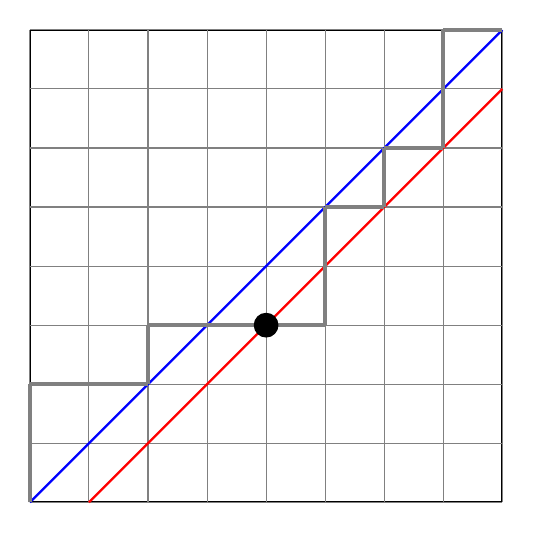
\begin{tikzpicture}[every plot/.style={mark=*, mark size=1.5mm, only marks}]
          \draw[step=6cm, thick] (0,0) grid (6cm,6cm);
          \draw[step=.75cm, gray] (0,0) grid (6cm,6cm);
          \draw[blue,thick] (0,0) -- (6cm,6cm);
          \draw[red,thick] (.75cm,0) -- (6cm, 7*.75cm);
          \draw[gray,ultra thick] (0,0) -- (0,2*.75cm);
          \draw[gray,ultra thick] (0,2*.75cm) -- (2*.75cm,2*.75cm);
          \draw[gray,ultra thick] (2*.75cm,2*.75cm) -- (2*.75cm,3*.75cm);
          \draw[gray,ultra thick] (2*.75cm,3*.75cm) -- (5*.75cm,3*.75cm);
          \draw[gray,ultra thick] (5*.75cm,3*.75cm) -- (5*.75cm,5*.75cm);
          \draw[gray,ultra thick] (5*.75cm,5*.75cm) -- (6*.75cm,5*.75cm);
          \draw[gray,ultra thick] (6*.75cm,5*.75cm) -- (6*.75cm,6*.75cm);
          \draw[gray,ultra thick] (6*.75cm,6*.75cm) -- (7*.75cm,6*.75cm);
          \draw[gray,ultra thick] (7*.75cm,6*.75cm) -- (7*.75cm,8*.75cm);
          \draw[gray,ultra thick] (7*.75cm,8*.75cm) -- (8*.75cm,8*.75cm);
          \draw plot coordinates{(4*.75cm,3*.75cm)};
        \end{tikzpicture}
        \caption{En av våra dåliga stigar, med huvuddiagonalen i blått och första diagonalen under huvuddiagonalen i rött. Punkten där stigen träffar den första underdiagonalen markeras med en cirkel.}
    \end{figure}

    Givet en dålig stig markerar vi första punkten på vilken den träffar första underdiagonalen, alltså diagonalen under huvuddiagonalen. Att det måste finnas en sådan punkt följer av att stigen är dålig -- om den aldrig träffade den underdiagonalen vore stigen en Dyckstig.

    Sedan speglar vi resten av stigen, efter punkten vi markerade, i första underdiagonalen. Vi ersätter alltså varje steg uppåt med ett steg till höger, och varje steg till höger med ett steg uppåt. 

    \begin{figure}\label{fig:dyck_comb_proof_reflected_path}
        \centering
        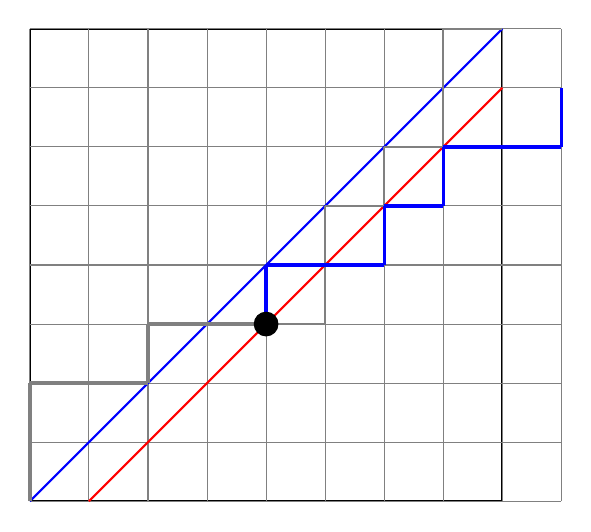
\begin{tikzpicture}[every plot/.style={mark=*, mark size=1.5mm, only marks}]
          \draw[step=6cm, thick] (0,0) grid (6cm,6cm);
          \draw[step=.75cm, gray] (0,0) grid (6.75cm,6cm);
          \draw[blue,thick] (0,0) -- (6cm,6cm);
          \draw[red,thick] (.75cm,0) -- (6cm, 7*.75cm);
          \draw[gray,ultra thick] (0,0) -- (0,2*.75cm);
          \draw[gray,ultra thick] (0,2*.75cm) -- (2*.75cm,2*.75cm);
          \draw[gray,ultra thick] (2*.75cm,2*.75cm) -- (2*.75cm,3*.75cm);
          \draw[gray,ultra thick] (2*.75cm,3*.75cm) -- (4*.75cm,3*.75cm);
          \draw[gray,thick] (2*.75cm,3*.75cm) -- (5*.75cm,3*.75cm);
          \draw[gray,thick] (5*.75cm,3*.75cm) -- (5*.75cm,5*.75cm);
          \draw[gray,thick] (5*.75cm,5*.75cm) -- (6*.75cm,5*.75cm);
          \draw[gray,thick] (6*.75cm,5*.75cm) -- (6*.75cm,6*.75cm);
          \draw[gray,thick] (6*.75cm,6*.75cm) -- (7*.75cm,6*.75cm);
          \draw[gray,thick] (7*.75cm,6*.75cm) -- (7*.75cm,8*.75cm);
          \draw[gray,thick] (7*.75cm,8*.75cm) -- (8*.75cm,8*.75cm);
          \draw[blue,very thick] (4*.75cm,3*.75cm) -- (4*.75cm,4*.75cm);
          \draw[blue,very thick] (4*.75cm,4*.75cm) -- (6*.75cm,4*.75cm);
          \draw[blue,very thick] (6*.75cm,4*.75cm) -- (6*.75cm,5*.75cm);
          \draw[blue,very thick] (6*.75cm,5*.75cm) -- (7*.75cm,5*.75cm);
          \draw[blue,very thick] (7*.75cm,5*.75cm) -- (7*.75cm,6*.75cm);
          \draw[blue,very thick] (7*.75cm,6*.75cm) -- (9*.75cm,6*.75cm);
          \draw[blue,very thick] (9*.75cm,6*.75cm) -- (9*.75cm,7*.75cm);
          \draw plot coordinates{(4*.75cm,3*.75cm)};
        \end{tikzpicture}
        \caption{Den uppåt-höger-stig från $(0,0)$ till $(n+1,n-1)$ som motsvarar vår dåliga stig i förra figuren. Stigen är grå fram tills punkten där vi började spegla den, och fortsätter sedan i blått. Originalstigen fortsätter i grått.}
    \end{figure}

    Eftersom vi i punkten vi började spegla just träffat första underdiagonalen så måste vi i den punkten ha haft ett steg mer åt höger än uppåt. Totalt har vi, i originalstigen, lika många steg uppåt som åt höger, så återstoden av den efter den punkten måste ha ett steg mer uppåt än åt höger.

    När vi speglar blir varje steg uppåt ett åt höger, och vice versa, så vår speglade stig måste ha ett steg mer åt höger än uppåt också i biten efter speglingen. Alltså måste den resulterande stigen efter speglingen ha två steg fler åt höger än uppåt, och alltså hamna i $(n+1,n-1)$.\sidenote[][-1cm]{I symboler har vi $u_i$ steg \emph{u}ppåt i stigen \emph{i}nnan punkten vi speglar efter, och $h_i$ steg åt \emph{h}öger. Efter punkten vi speglar \emph{e}fter har vi $u_e$ steg uppåt och $h_e$ steg åt höger. Så i Figur \ref{fig:dyck_comb_proof_path} så har vi $u_i = 3$, $h_i = 4$, $u_e = 5$, och $h_e = 4$.
    
    Så för stigen vi börjar med har vi $h_i = u_i + 1$, och $h_i + h_e = n$ samt $u_i + u_e = n$ för att den skall sluta i $(n,n)$. Stigen efter speglingen kommer att ha $h_i + u_e$ steg åt höger och $u_i + h_e$ steg uppåt. Om man arbetar sig igenom dessa ekvationer kommer man att se att vi verkligen har $n+1$ steg åt höger och $n-1$ steg uppåt i den reflekterade stigen.}

    Så vi har hittat ett sätt att skicka en dålig stig på en stig från $(0,0)$ till $(n+1,n-1)$. För att detta skall vara en bijektion måste processen vara reversibel - givet en stig från $(0,0)$ till $(n+1,n-1)$ måste vi kunna återskapa den motsvarande dåliga stigen.

    Sättet vi gör det på är samma som innan -- vi hittar första punkten i vilken vår stig träffar första underdiagonalen, och speglar efter den. Att en sådan punkt måste finnas är uppenbart, eftersom $(0,0)$ ligger ovanför den underdiagonalen, och $(n+1,n-1)$ ligger under den. Så för att ta oss från ena sidan av den till andra måste vi passera den.

    Att denna spegling kommer ge oss rätt dåliga stig är enkelt att se -- allt vi gjort är att spegla två gånger, vilket så klart inte gör någonting.

    Alltså har vi bevisat att antalet dåliga stigar är lika med antalet stigar från $(0,0)$ till $(n+1,n-1)$. Vi vet att det finns $\binom{(n + 1) + (n - 1)}{n+1}$ sådana stigar, så vi kan räkna att
    \begin{align*}
        d_n &= \abs{\text{stigar }(0,0)\to(n,n)} - \abs{\text{dåliga stigar}}\\
        &= \binom{2n}{n} - \binom{2n}{n+1}\\
        &= \frac{(2n)!}{n!n!} - \frac{(2n)!}{(n+1)!(n-1)!}\\
        &= (2n)!\left(\frac{(n+1)}{(n+1)!n!} - \frac{n}{(n+1)!n!}\right)\\
        &= \frac{(2n)!}{(n+1)!n!} = \frac{1}{n+1}\frac{(2n)!}{n!n!} = \frac{1}{n+1}\binom{2n}{n}
    \end{align*}
    vilket bevisar satsen.
\end{proof}

Så vårt kombinatoriska bevis undvek helt att behöva fundera på rekursioner och genererande funktioner. Det är en mycket mer direkt rutt till vårt mål, men vi missade några sevärdheter längs vägen.\sidenote[][]{Hur man hade härlett vår rekursion eller den genererande funktionen givet bara vad vi lärde oss i det kombinatoriska beviset är långt ifrån uppenbart.}

\section{Fler saker som räknas av Catalantalen}

Som vi nämnde tidigare är Catalantalen viktiga eftersom de räknar fler saker än bara just Dyck-stigar. I nästa föreläsning kommer vi se ett viktigt exempel. Nu, i slutet på denna, tar vi några mindre exempel.

\begin{example}
    Antalet sätt att skriva $2n$ matchande parenteser räknas av Catalantalen. Med matchande parenteser menar vi alltså ett uttryck som $(()(()))()(())$ -- och i ett uttryck som $)((()$ matchar de inte. Varje $($ måste ha en motsvarande $)$ senare i ordet, och varje $)$ måste ha ett matchande $($ senare i ordet.

    Hur bevisar vi att detta räknas av Catalantalen? Jo, vi ser att detta lyder samma rekursion som Dyck-stigarna gjorde. Varje uttryck med matchande parenteser måste börja med $($, och denna första startparentes måste matcha en slutparentes. Det som står inom dessa parenteser måste också vara ett matchande uttryck, och likaså det som står efter slutparentesen som matchar första parentesen.

    Alltså kan vi skriva varje uttryck med matchande parenteser på formen $(w_1)w_2$, med $w_1$ och $w_2$ två kortare matchande uttryck. Det här är precis samma uppdelning som vi hade för våra Dyckstigar, så det kommer ge samma rekursion, och alltså är det samma följd.\sidenote[][-2cm]{Vi hade också, vilket kanske vore enklare, helt enkelt kunnat se att det finns en bijektion mellan matchande uttryck med parenteser och Dyck-stigar, genom att tolka $($ som ``steg uppåt'' och $)$ som ``steg till höger''.}
\end{example}

\begin{example}\label{example_polygons}
    Det problem som ursprungligen fick upp matematikers intresse i väst\sidenote[][-0.6cm]{De studerades först av en matematiker i Kina på 1700-talet vid namn Minggatu, som använde dem för att ge identiteter för sinus-funktionen, i stil med
    $$\sin(2\alpha) = 2\sin(\alpha) - \sum_{n=1}^{\infty} \frac{C_{n-1}}{4^{n-1}}\sin^{2n+1}(\alpha).$$} för Catalantalen var att dela upp en konvex polygon med $n+2$ sidor i trianglar, genom att rita streck mellan hörnen som inte korsar varandra.

    \begin{figure}
        \centering
        \includegraphics[width = 0.5\textwidth]{graphics/Catalan-Hexagons-example.pdf}
        \caption{Fallet med hexagoner.}
    \end{figure}

    Det här problemet studerades först av Euler\sidenote[][]{Som ju redan har mer än tillräckligt med saker namngivna efter sig, så det är tur att vi inte döpte talen efter honom.}, och beviset att de räknas av Catalantalen utvecklades av Segner, Goldbach, och Lamé. Vår rekursion för Catalantalen brukar kallas för Segnerrekursionen.

    Senare studerades problemet med parentetiseringar av Eugène Charles Catalan, efter vilken talen fick sitt namn på femtiotalet.
\end{example}

\section{Övningar}

\begin{xca}
    Hur många gitterstigar av längd $n$ från $(0,0)$ till $(a,b)$ finns det?
\end{xca}

\begin{xca}
    Bevisa att antalet uppdelningar av en konvex polygon med $n+2$ sidor i trianglar, såsom vi diskuterade i Exempel \ref{example_polygons}, räknas av Catalantalen.\sidenote[][]{Ledtråd: Tänk kombinatoriskt, och se att dessa också lyder vår rekursion.}
\end{xca}

\bibliography{references}
\bibliographystyle{plainnat}

\end{document}
